\section{Weighing an Electron}

\makelabheader %(Space for student name, etc., defined in master.tex)

\bigskip
\textbf{Objective}

To investigate the force on a charged particle due to a magnetic field and 
learn how the motion of the particle can be used to weigh it.

\bigskip
\textbf{Apparatus}

\begin{itemize}[nosep]

\item $e/m$ apparatus

\item Low- and high-voltage power supplies

\item Two digital multimeters

\item Ruler

\item Flashlight

\end{itemize}

\medskip
\textbf{Overview}

Mass spectroscopy is an experimental technique that is used to determine
the mass of atoms, molecules, and sub-atomic particles.
The central idea is to make a version of the particle carrying an electric
charge ({\it e.g.}, a bare electron, an ionized molecule, {\it etc}), accelerate it
through an electric potential, and then inject it into a magnetic field.
If properly oriented, the magnetic field will bend the particle's trajectory into
a curved path.
The amount of curvature depends on the particle's electric
charge and its mass, so that the paths of different mass particles with the same charge will
bend by different amounts.
Measuring this bend is equivalent to a mass measurement.
This method is widely used to do things like determine the mass of newly discovered particles,
hunt for oil, and even validate the authenticity of works of art.

\bigskip
\textbf{Activity 1: Magnetic Force on a Charged Particle}

It has been found by careful measurements that the force $\vec F_B$ on a charged
particle due to a magnetic field is
\begin{equation}
\vec F_B = q \vec v \times \vec B
\end{equation}
where $q$ is the electric charge of the particle, $\vec v$ is its velocity,
and $\vec B$ is the local magnetic field.
(If necessary, you can find the relevant sections in your text for a discussion of the cross product.)

\begin{enumerate}[labparts]
\item In the figure below, a uniform magnetic field $\vec B$ points out of the page (in the $z$ direction), and a particle of charge $q$ moves to the right as shown.  What is the direction of the force $\vec F_B$ on the particle if $q$ is \textit{positive}?

\medskip
\hspace{0.5in}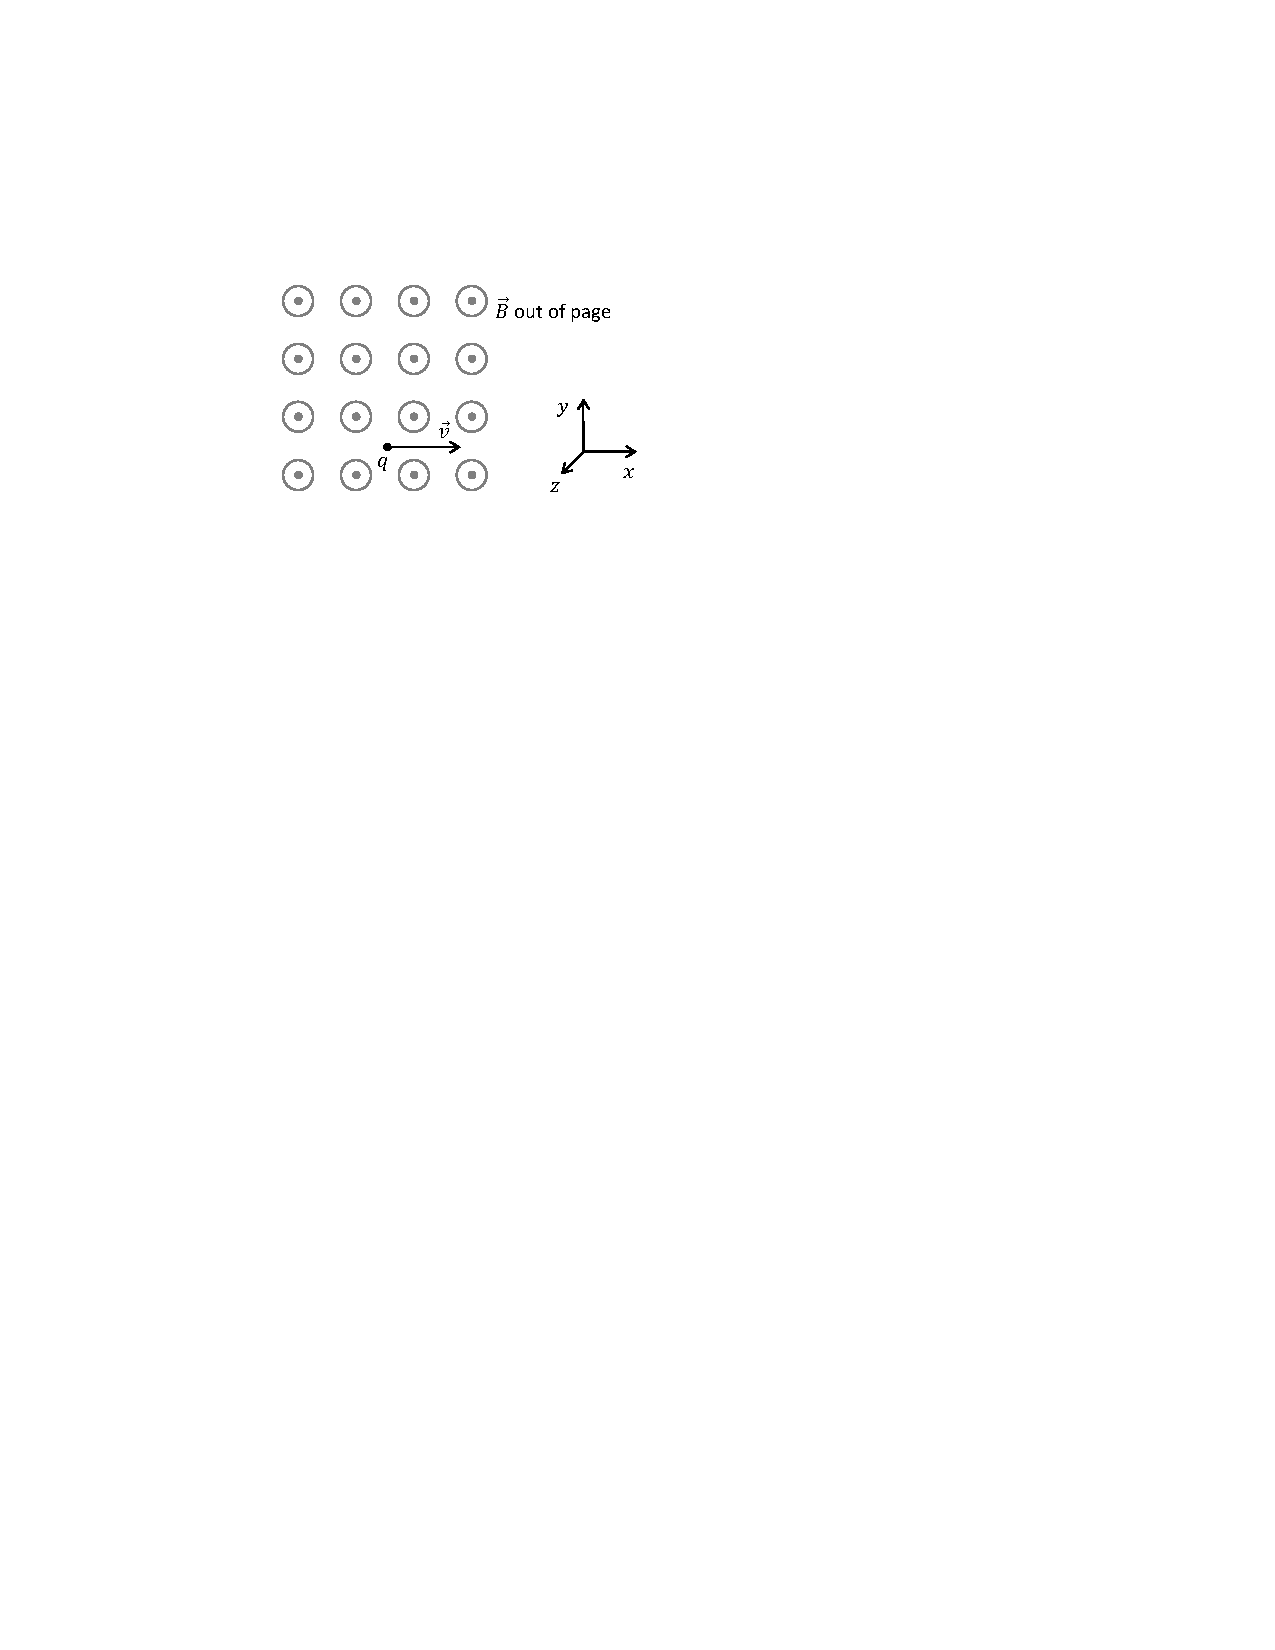
\includegraphics{eoverm/q_in_field1.pdf}
\medskip

\item In the same figure above, what is the direction of the force $\vec F_B$ on the particle if $q$ is \textit{negative}?
\answerspace{0.5in}


\pagebreak[2]
\item At some later time, the same \textit{negatively} charged particle has been steered to the new position shown below, with velocity $\vec v$ now in the $+y$ direction.  Now what is the direction of the force $\vec F_B$ on the particle?

\medskip
\hspace{0.5in}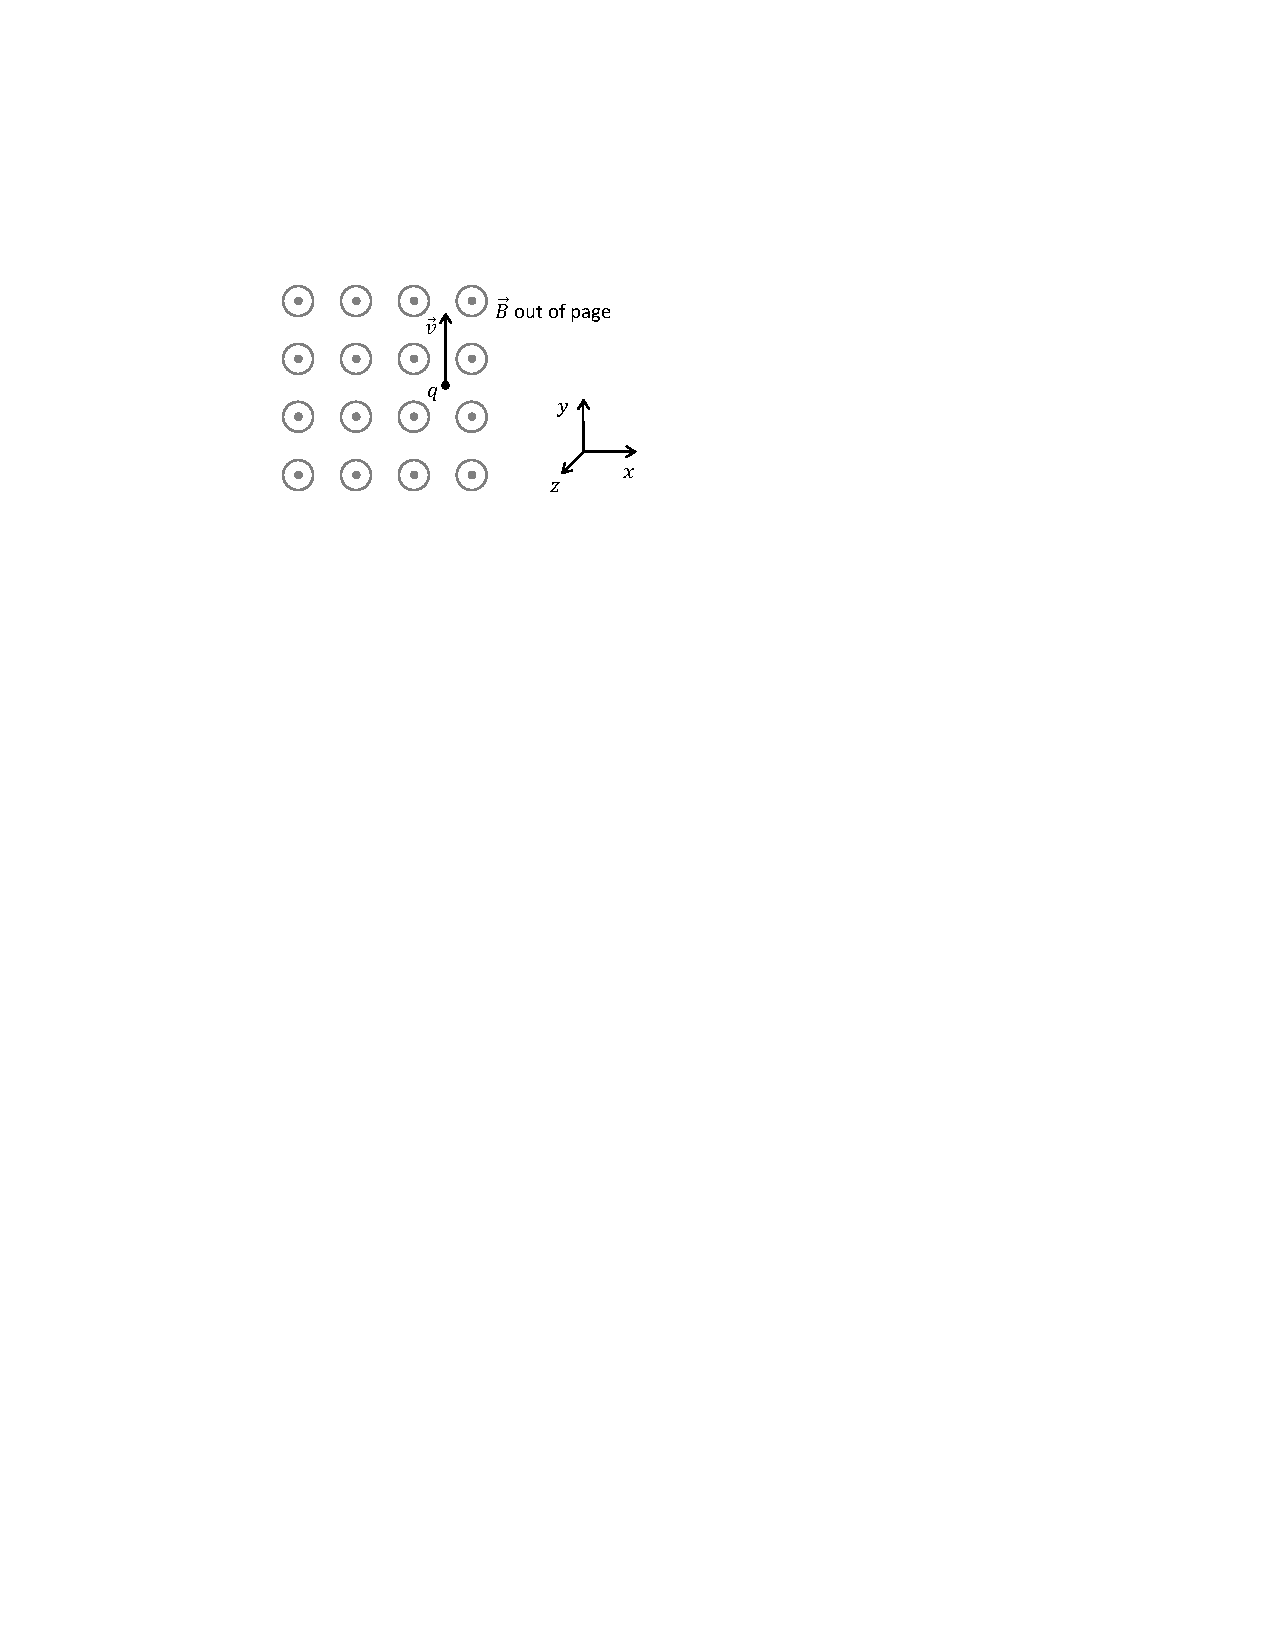
\includegraphics{eoverm/q_in_field2.pdf}
\medskip

\item In general, from Equation (1), how is the magnitude of the cross product $\vec v \times \vec B$ related to
the magnitudes $v$ and $B$ and the angle $\theta$ between $\vec v$ 
and $\vec B$?
\answerspace{0.5in}

\item For the specific case of the particle in the picture above, what is the magnitude of the force $F_B$ on the particle in terms of $|q|$, $v$, and $B$? (Hint: what is the angle $\theta$ between $\vec v$ and $\vec B$?)  Does that magnitude change?  
\answerspace{0.5in}

\item Describe the trajectory of the charged particle.
What is the $z$ component of its trajectory?
\answerspace{0.5in}

\item How are the directions of $\vec F_B$ and $\vec v$ related?
\answerspace{0.5in}
\end{enumerate}


%\begin{figure}[!hb]
%\begin{center}
%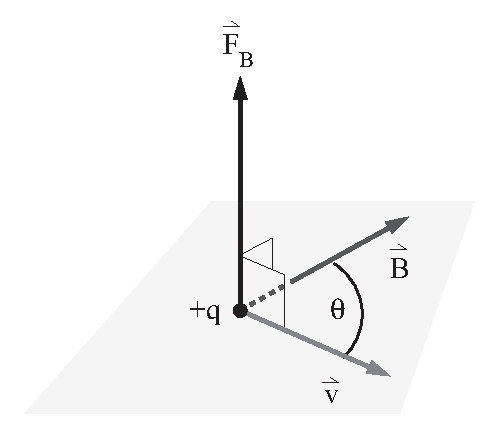
\includegraphics[height=2.0in]{eoverm/vCrossB_bw.eps}
%\caption{Vectors associated with the magnetic force. \hfill}
%\end{center}
%\end{figure}


\textbf{Activity 2: Relating $\vec F_B$ to the Kinematics}

In the previous section you should have found that the charged particle moves in a circular path in the $xy$ plane.  The magnetic force $\vec F_B$ is always perpendicular to $\vec v$,  with a constant magnitude $F_B = |qvB|$.  Here, $\vec F_B$ is the \textit{only} force acting on the particle, and it plays the role of the \textit{centripetal} force in the uniform circular motion of the particle.

\begin{enumerate}[labparts]

%(a) What type of force have we encountered 
%that is perpendicular to the velocity and constant in magnitude?
%(Hint: Recall some of the applications of Newton's Laws in your text.)
%\vspace{15mm}

\item How is centripetal acceleration $a_c$ related to $v$ and $r$ (the radius of the
circular motion)? From Newton's 2nd Law, what is the expression for the magnitude of the centripetal force $|\vec F_c|$ in terms of $v$, $r$, and $m$?
\answerspace{15mm}


\item Since the magnetic force $\vec F_B$ and the centripetal force $\vec F_c$ are the same thing here, set their magnitudes equal to each other, using your expression for $F_B$ from Activity 1, and your expression for $F_c$ from above.  
Solve for the mass $m$ of the particle in terms of the radius $r$ of the particle's path,
$|q|$, $v$, and $B$. \label{eoverm_m_qvB}
\answerspace{35mm}


\item For two particles with the same charge and velocity, but different masses, which one will have the larger path radius?
\answerspace{0.5in}

\item How would increasing the velocity of a particle change the radius of its path?  \label{eoverm_predict_radius}
\answerspace{0.5in}

\item In a mass spectrometer, the particle is first accelerated
across an electric potential difference. Typically, we know the kinetic 
energy $K$ of the charged particle after this acceleration instead of the 
velocity. Rewrite your result in 2\ref{eoverm_m_qvB} in terms of the kinetic energy $K$ 
instead of the velocity $v$. (To do this, solve the kinetic energy equation for velocity, 
and substitute it for $v$ in the result of 2\ref{eoverm_m_qvB}. Then solve the result to isolate $m$ on one side.) \label{eoverm_m_qBrK}
\answerspace{30mm}

\item In the experiment you will do, the electron of charge $e$ ``falls'' across a potential difference created by the 
accelerating voltage to gain a velocity $v$ before it enters the magnetic 
field region. Assuming the electron starts from rest, what is the relationship 
between the accelerating voltage $V$ and the kinetic energy $K$ when it leaves the 
accelerating region and enters the magnetic field? (Use conservation of energy 
to determine this.) Combine this withyour result from part~2\ref{eoverm_m_qBrK} to get an 
expression for the mass $m$ of the electron in terms of
$V$, $r$, $B$, and the electron charge $e$. \label{eoverm_m_eBrV}
\answerspace{50mm}

%(f) We will use the mass spectrometer to measure the radius of the particle's trajectory
%and then derive a mass from that measurement. Rearrange your result from
%section 2.e to isolate the mass $m$ on one side of the equation.
%\vspace{30mm}

\end{enumerate}

\pagebreak[3]

\vspace*{0.2in}

\textbf{Activity 3: Measuring a Charged Particle in a Magnetic Field}


\begin{wrapfigure}{r}{3.2in}
\begin{center}
\vspace{-0.5in}
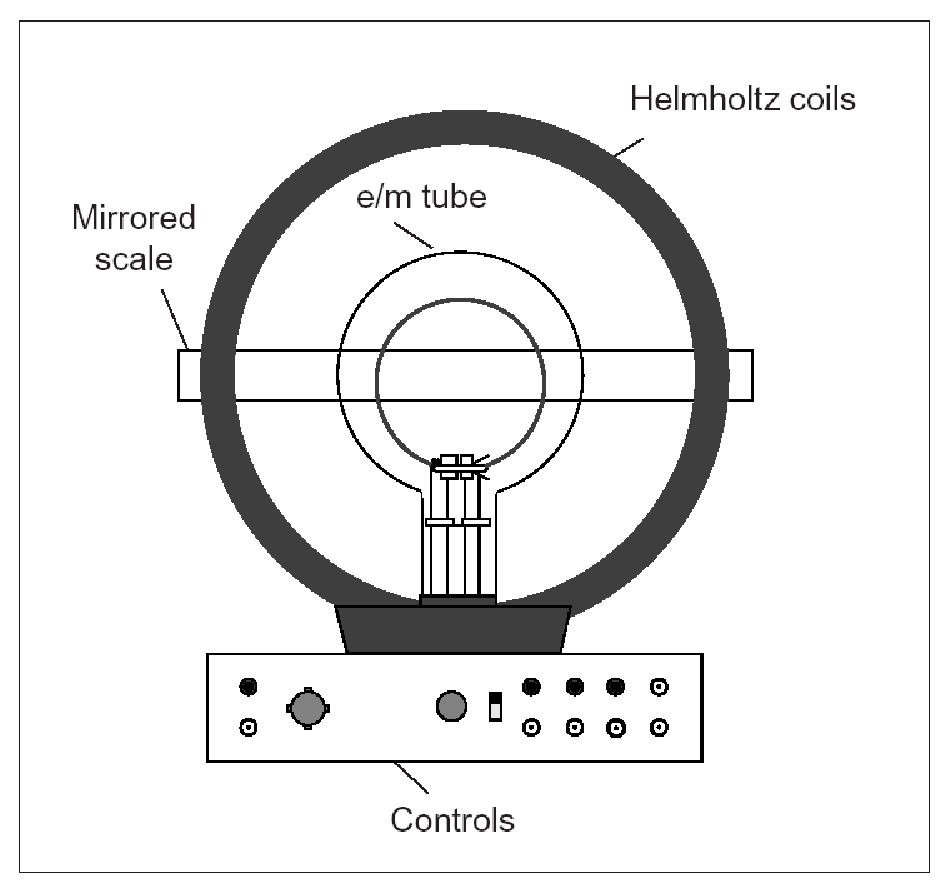
\includegraphics[trim=2mm 2mm 2mm 2mm, clip, height=3.0in]{eoverm/apparatus1.eps}
%\caption{The $e/m$ apparatus.}
The $e/m$ apparatus
\end{center}
\end{wrapfigure}

\bigskip\bigskip

The last piece of the puzzle before we start measuring things is the magnetic 
field $\vec B$. The apparatus you are using consists of a pair of wire coils 
(called Helmholtz coils) and an electron gun that produces a beam of electrons.
From the picture to the right, identify the Helmholtz coils on your $e/m$ apparatus.\footnote{What you are doing is often called the $e/m$ (``$e$ over $m$'') experiment, first done by J. J.~Thomson in 1897.  At the time, the charge $e$ of the electron was unknown, so Thomson couldn't measure $m$ independently, but he could measure the charge-to-mass ratio $e/m$.   The charge $e$ of the electron was later measured by Robert A. Millikan in 1909.}


The magnitude of the magnetic field along the axis of the pair of coils is
\begin{equation}
B = \left ( \frac{4}{5} \right )^{3/2} \frac{N \mu_0 I}{a}
\end{equation}
where $N$ is the number of turns of wire in each coil, $\mu_0$
is the permeability constant,  $I$ is the current in the coils,
and $a$ is the radius of the coil.
The direction of the field is parallel or anti-parallel
to the axis of the pair of coils depending on the direction of the current
in the coils.
The direction of the current is the same in each coil.
The magnetic field in the region between the coils is approximately equal
to the field along the axis of the coils so we will use
the expression above for our magnetic field in the equation you generated in
part~2\ref{eoverm_m_eBrV}.

\bigskip

\begin{enumerate}[labparts]

\item The number of turns of wire in each Helmholtz coil is $N=130$. Notice that 
the turns on each coil are wrapped on top of one another, so the radii of the 
turns are not all the same. We will approximate an average value by measuring 
the diameter of the coils from the center of the housing on one side to the 
center of the housing on the other side. Record that diameter and the value of 
$a$ (half the diameter) here:
\answerspace{0.4in}

\item Now calculate the magnetic field $B$ due to the Helmholtz coils using equation 
(2), assuming a current of 1.50 amperes in the coils. Show that the result is 
in $tesla$.
\answerspace{1.5in}

\pagebreak[3]

\item Identify each item on the front panel below
the Helmholtz coils, using the connection diagram below as a guide.
Check that all the connections are correct on your setup. 

\begin{center}
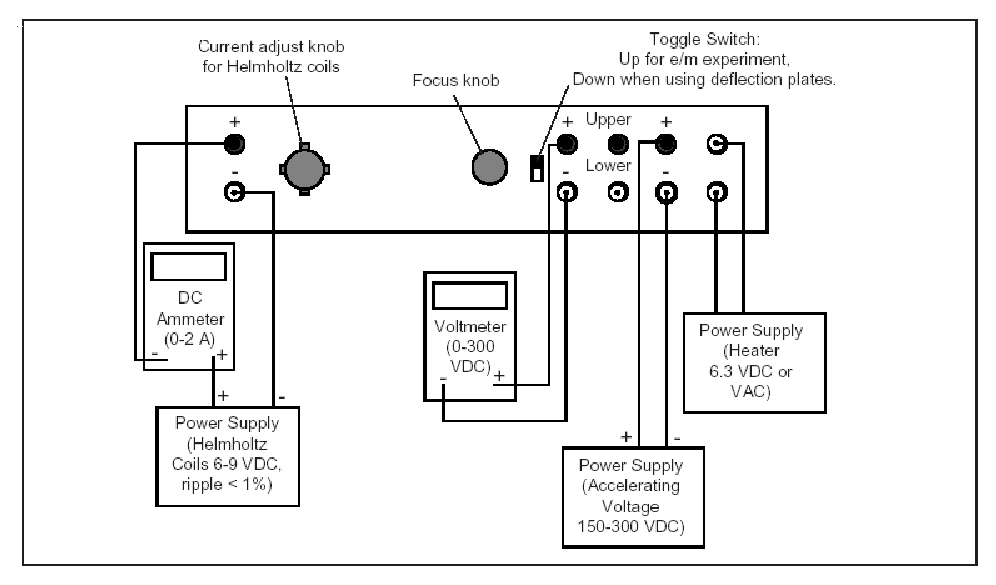
\includegraphics[trim=2mm 2mm 2mm 2mm, clip, height=3.5in]{eoverm/apparatus2.eps}

%\caption{Instrument connections for the e/m experiment.}
Connection diagram for the e/m experiment

\end{center}

\item Place the hood over the $e/m$ apparatus and flip the 
toggle switch up to the $e/m$ MEASURE
position.
Turn the current adjust knob for the Helmholtz coils to the vertical position (white line
at the 12 o'clock noon position).

\item Identify the ammeter used to measure the current in the Helmholtz
coils using the connection diagram above as a guide. 
Next, turn on the low-voltage power supply for the Helmholtz coils.
Now watch the current in the ammeter (it should not exceed $2$~A under
any circumstances) and
turn up the voltage on the Helmholtz coils into the range of $6-9$~V.

\item As you watch the ammeter slowly turn the current adjust knob for the 
Helmholtz coils clockwise. Take care that
the current in the ammeter does not exceed 2~A.
Set the current adjust knob for the Helmholtz coils to 1.50~A.

\item Identify the power supply that runs the heater for the electron gun using 
the connection diagram above as a guide and turn on the power supply. Turn the voltage up to 
6 volts. {\bf CAUTION:} Do not exceed 6 volts or you may destroy the $e/m$
tube.

\item Turn on the power supply for the accelerating voltage for the electron gun.
Turn the voltage up so that it is in the range of 150 -- 160~V.

\item Wait several minutes for the cathode to heat up. When
it does, you will see the electron beam emerge from
the electron gun and it will be curved by the field from
the Helmholtz coils. If the electron beam is not sharp, adjust the focus knob. 
Check that the electron beam is
parallel to the Helmholtz coils. If it is not, consult your instructor.
 Carefully read the current in the Helmholtz coils from
your ammeter and the accelerating voltage from your
voltmeter. Record the values on one line in the table on the following page.
\label{eoverm_B1.5amps}

\begin{minipage}{0.55\textwidth}

\item Carefully measure the radius of the electron beam.
To avoid parallax errors, move your head to align one side of the electron
beam with its reflection, as shown to the right, and read the radius from the scale.
Because the entire tube may be slightly off center, you should record the apparent radius from both the left and right sides, then take their average. 
Record your results in one row of the table below. \label{eoverm_parallax}
%\answerspace{2in}
\end{minipage}
\begin{minipage}{0.44\textwidth}
%\vspace{-0.5in}
\hfill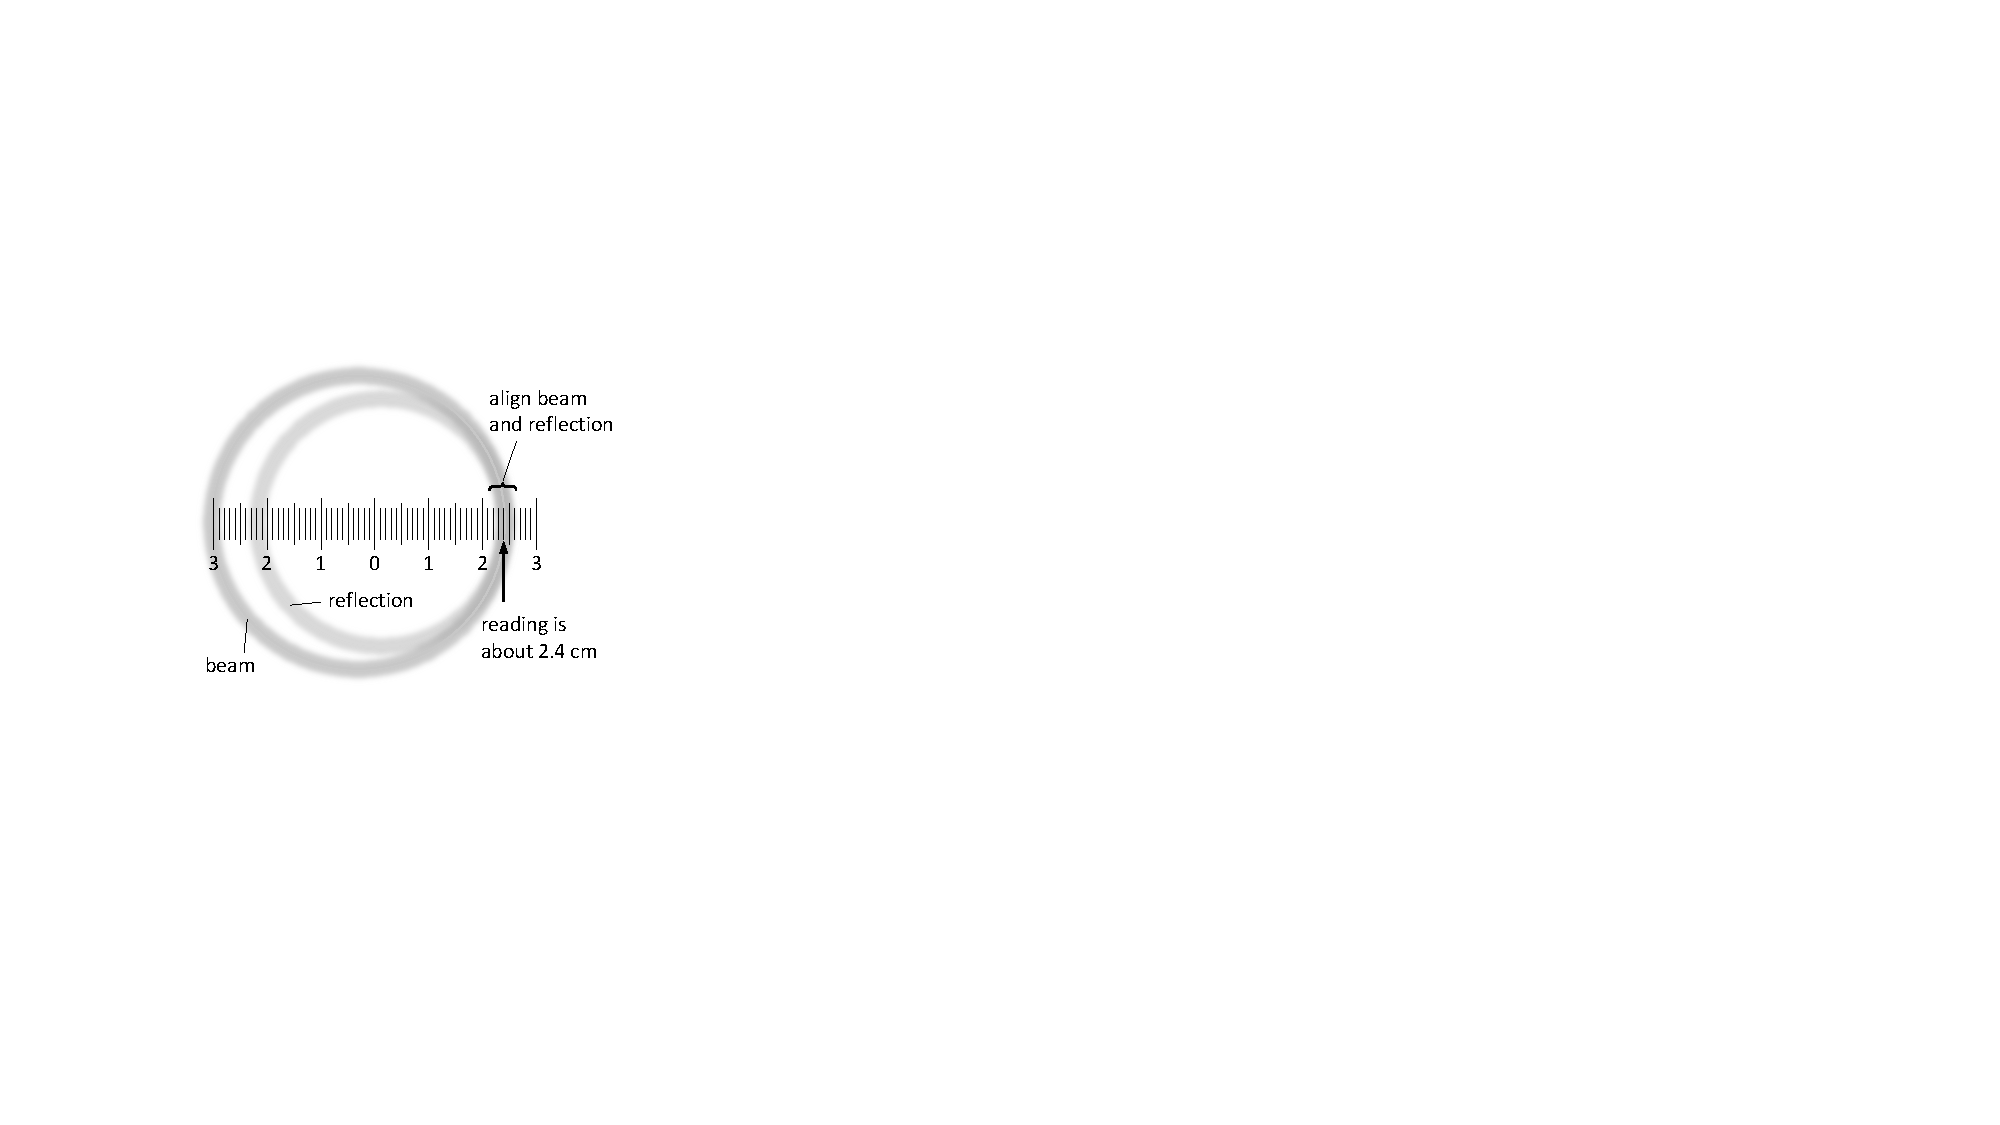
\includegraphics[scale=0.9]{eoverm/aligning_beam_and_reflection.pdf}

\end{minipage}

\item Slowly turn the current adjust knob for the Helmholtz
coils either up or down as you watch the ammeter and take care that
the current does not exceed 2~A.
What parameter does this action affect, the magnetic field or the
accelerating voltage?
What happens to the path of the electrons as the current in the Helmholtz
coils changes? Does this agree with what you expected? Explain.
%Set the current adjust knob to some value and
%repeat parts 4.h-i to get a second measurement. Record the current in the
%Helmholtz coils, the accelerating voltage, and the average radius of the electron beam.
\answerspace{20mm}

%(k) Slowly change the accelerating voltage either up or down.
%What parameter does this voltage effect? Consider your result for part 2.f.
%What happens to the electron's path?
%Set the accelerating voltage 
%to some value and
%repeat parts 4.h-i to get a third measurement. Record the current in the
%Helmholtz coils, the accelerating voltage, and the average radius of the electron beam.
 \item Return the current in the Helmholtz coils to the value you recorded in 
part~\ref{eoverm_B1.5amps} ($\approx 1.50$~A). Slowly increase the accelerating voltage. What parameter 
does this voltage affect? What happens to the electron's path?  Does this agree with your prediction in part~2\ref{eoverm_predict_radius}?
\answerspace{0.5in}

\item Take a few more readings for different values of the accelerating voltage (say at least one lower than 150~V
 and one higher).  In the table below, record the accelerating voltage, the current in the 
Helmholtz coils (could be the same for all) 
and the average radius of the electron beam (by measuring the radius of the 
beam on both sides of the scale and averaging as you did in part~\ref{eoverm_parallax} above). 

\begin{center}
{\renewcommand{\arraystretch}{1.8}
\begin{tabular}{|*{7}{ C{0.75in} |}}
\hline
$V$ & $I$ & $B$ & $r_{\rm left}$ & $r_{\rm right}$ & $r_{\rm avg}$ & $m_e$  \\ 
\hhline{|=|=|=|=|=|=|=|}
& & & & & & \\ \hline
& & & & & & \\ \hline
& & & & & & \\ \hline
& & & & & & \\ \hline
& & & & & & \\ \hline
\end{tabular}
}
\end{center}

\item When you are finished with your measurements, turn down to zero the accelerating voltage, the 
heater voltage, the Helmholtz coil voltage, and the current adjust knob.

\end{enumerate}

\pagebreak[2]
\textbf{Activity 4: Extracting the Electron Mass From Your Data}

\begin{enumerate}[labparts]

\item For each row of your data table, calculate the magnetic field in the coils $B$ and the apparent mass of the electron $m_e$ from your data.  (The accepted mass of the electron is $m_e = 9.1094 \times 10^{-31}$~kg.  You might want to double check your units if you're not at least somewhere in the ballpark.)
\answerspace{1.5in}

\item Now let's calculate the uncertainty in $m_e$ for one of your measurements.  There are at least three measured quantities in your data table that could contain uncertainty.  In the space below, write the values of those measurements along with estimates of their uncertainties (in the form $x \pm \delta x$) for one row of your data table.  You can assume that measurements from your multimeters are accurate to about 1\% in the ranges you used them.
\answerspace{1.5in}

\item For each of the quantities you just listed, calculate the uncertainty $\delta m_e$ in your electron mass due to the uncertainty in \textit{just that one} measured quantity.  (See Appendix~\ref{uncertainty} if needed.)
\answerspace{1.5in}

\item Combine your results above to calculate an overall uncertainty for one of your measurements of the electron mass, and state your final result for $m_e \pm \delta m_e$ here.   Does the accepted value fall within your range?  Are there other uncertainties in your measurements that you didn't account for? 
\answerspace{0.5in}

\end{enumerate}


%\begin{table}[h!]
%\begin{center}
%\begin{tabular}{|l|c|l|c|l|c|} \hline
%\hi Particle         & mass ($MeV/c^2$)  & Particle             & mass ($MeV/c^2$)  & Particle             & mass ($MeV/c^2$) \\ \hline
%\hi electron($e^-$)  & 0.511             & u-quark($u$)         & 1.5-4.0           & $\rm ^{12}C$         & 11,178 \\[2pt] \hline
%\hi positron($e^+$)  & 0.511             & neutrino($\nu_\tau$) & < 18.2            & $\rm ^{16}O$         & 14,904 \\[2pt] \hline
%\hi proton           & 938.27            & neutrino($\nu_e$)    & < 0.000003        & muon($\mu^+$)        & 105.66 \\[2pt] \hline
%\hi neutron          & 939.57            & neutrino($\nu_\mu$)  & < 0.19            & pion($\pi^+$)        & 139.57 \\[2pt] \hline
%\hi muon($\mu^-$)    & 105.66            & tau($\tau^-$)        & 1,777.0           & pion($\pi^-$)        & 139.57 \\[2pt] \hline
%\end{tabular}
%\caption{Some  particle masses.}
%\end{center}
%\end{table}

%\begin{table}[h!]
%\begin{center}
%\begin{tabular}{|l|c|l|c|} \hline
%\hi Particle         & mass ($MeV/c^2$)  & Particle             & mass ($MeV/c^2$) \\ \hline
%\hi electron($e^-$)  & 0.511             & $\rm ^{12}C$         & 11,178 \\[2pt] \hline
%\hi positron($e^+$)  & 0.511             & $\rm ^{16}O$         & 14,904 \\[2pt] \hline
%\hi proton           & 938.27            & muon($\mu^+$)        & 105.66 \\[2pt] \hline
%\hi neutron          & 939.57            & pion($\pi^+$)        & 139.57 \\[2pt] \hline
%\hi muon($\mu^-$)    & 105.66            & tau($\tau^-$)        & 1,777.0 \\[2pt] \hline
%\hi neutrino($\nu_e$)& < 0.000003        & neutrino($\nu_\mu$)  & < 0.19 \\[2pt] \hline
%\hi u-quark($u$)     & 1.5-4.0           & neutrino($\nu_\tau$) & < 18.2 \\[2pt] \hline
%\end{tabular}
%\caption{Some atomic and sub-atomic particle masses.}
%\end{center}
%\end{table}

